
\documentclass[9pt]{beamer}
\usepackage[english]{babel}
\usepackage{amsfonts}
\usepackage{array}
\usepackage{amsmath}
\usepackage{amssymb}
\usepackage{natbib}
\usepackage{caption}
\usepackage{subcaption}
\usepackage{multirow}
\usepackage{multicol}
\usepackage{hyperref}
\usepackage{tikz}
\usetikzlibrary{arrows.meta, positioning}

\bibliographystyle{abbrvnatsimple} % The filename of the bibliography

\usepackage{threeparttable}
%\bibliographystyle{abbrvnat} % The filename of the bibliography
\setcitestyle{authoryear,open={(},close={)}} 
\usepackage[autostyle=true]{csquotes} % Required to generate language-dependent quotes in the bibliography
\usepackage{booktabs}
\usepackage{graphics}
\usepackage{svg}
\captionsetup[figure]{font=footnotesize}

\usepackage{appendixnumberbeamer} 

\title[Intro to ABMs]{Introduction to Agent-Based Models}

\author[S.G. Hoekstra]{Steven Hoekstra \inst{1} \inst{2} }
\institute[UvA]{\inst{1} CeNDEF, University of Amsterdam, 
                      \inst{2} Tinbergen Institute}


\date{}

\titlegraphic{

\includegraphics[width=5cm]{figs/uvalogo_g_en_Amsterdam_School_of_Economics.eps} 
}



\usetheme{Berlin} 
\usecolortheme{beaver}

\begin{document}

\begin{frame} 
    \maketitle
\end{frame}


\begin{frame}{Overview}
    \tableofcontents
    \note{    
    \begin{itemize}
        \item Welcome
        \item Tell about yourself
        \item Tell about today.
        \item Tell about the programming part in the end
    \end{itemize}
 }
 
\end{frame}
\section{Introduction}

\begin{frame}{Why Agent-Based Models?}
    \begin{itemize}
        \item<1-> Traditional models often revert to a steady state after a shock.
        \item<2-> ABMs can generate \textbf{persistent dynamics} and \textbf{path dependence}.
        \item<3-> This makes them suitable for forecasting and policy analysis.
    \end{itemize}
\begin{figure}
    \centering
    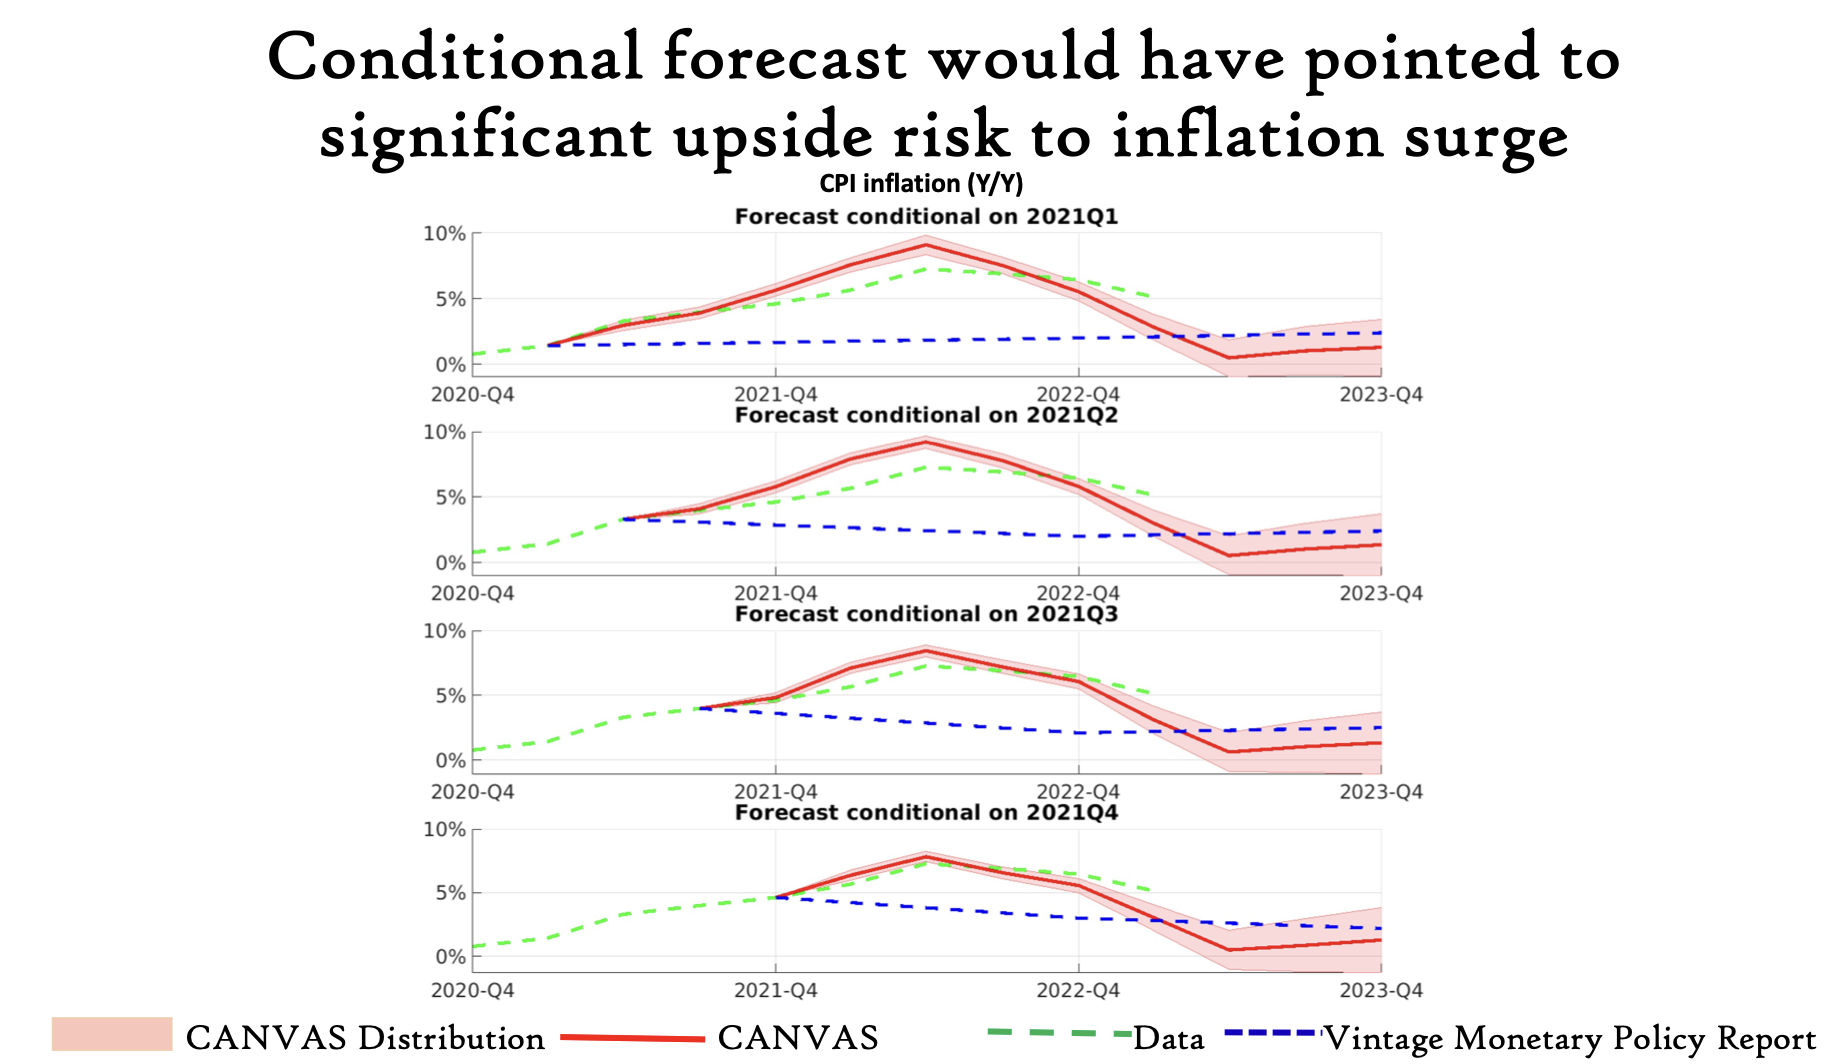
\includegraphics[width=0.8\linewidth]{figs/forecast_abm_vs_old.png}
    \caption{ABM inflation forecast vs traditional models. \citep{Canvas-presentation}}
\end{figure}
\end{frame}

\begin{frame}{ABMs vs.\ DSGE Models}
\begin{columns}[T]
\begin{column}{0.48\textwidth}
\textbf{DSGE (traditional)}
\begin{itemize}
  \item Representative agent
  \item Rational expectations
  \item Equilibrium dynamics
  \item Analytical / linearised solutions
  \item Exogenous shocks drive cycles
\end{itemize}
\end{column}
\begin{column}{0.48\textwidth}
\textbf{Agent-Based Models}
\begin{itemize}
  \item Heterogeneous agents
  \item Bounded rationality
  \item Out-of-equilibrium dynamics
  \item Computational simulation
  \item Endogenous crises can emerge
\end{itemize}
\end{column}
\end{columns}

\vspace{0.4cm}
ABMs and DSGE are \textbf{complementary}: DSGE excels at analytical tractability, ABMs provide flexibility to model heterogeneity, networks, and non-linear feedbacks.
\end{frame}

\begin{frame}{What are Agent Based Models (ABMs)?}
    \begin{itemize}
        \item<1-> \textbf{simulation-based modelling} approach
        \item<2-> \textbf{bottoms-up approach} instead of formula-based top-down approach.
        \item<3->  We can analyse systems, perform policy analysis and forecast with ABMs.
        \item<4-> ABMs can give insights which traditional models cannot.
        \begin{itemize}
            \item<5-> Forecast inflation distributions per sector.
            \item<6-> Stress test the \textbf{entire EU banking system} with a 1-1 ABM.
            \item<7-> Estimate the flood risk per firm/household for an entire country.
        \end{itemize}
        \item<8-> Widely applied in biology, physics, chemistry, sociology, and economics.
    \end{itemize}

    \note{    
    \begin{itemize}
        \item Agent-based models are a \textbf{simulation-based               modelling} approach to analyse social and economic phenomena.
    \item We can use agent-based models to analyse systems, ask what-if questions, and (recently) to forecast.
    \item Agent-based models use a \textbf{bottoms-up approach} instead of formula-based top-down approach simulating some or each individual of the system that we are interested.\\
    \item Agent-based models have been widely applied, including in biology, physics, chemistry, sociology, and economics. ABMs are becoming more popular in economics after the GFC.
    \end{itemize}
    
 }
\end{frame}



\begin{frame}{What are agent-based model typical elements?}
    \begin{columns}
\begin{column}{0.6\textwidth}
     \begin{itemize}
        \item<1-> Multiple agents
        \item<2-> In economics: households, firms, banks, government, and central bank.
        \item<3-> \textbf{Local} and/or \textbf{global} interaction
        \item<4-> Agents make decisions based on their state/information.
        \item<5-> Interaction based on \textbf{topology or network}.
        \item<6-> Environment in which agents are embedded in.
        \item<7-> Global (macro) dynamics are \textbf{emergent} from local (micro) interactions.
        \item<8-> Expectations are often \textbf{boundedly rational}.
        \item<9-> \href{https://www.youtube.com/watch?v=C2vgICfQawE&t=203s}{Conway's Game of Life}
    \end{itemize}
\end{column}
\begin{column}{0.4\textwidth}  
        \begin{figure}
        \centering
    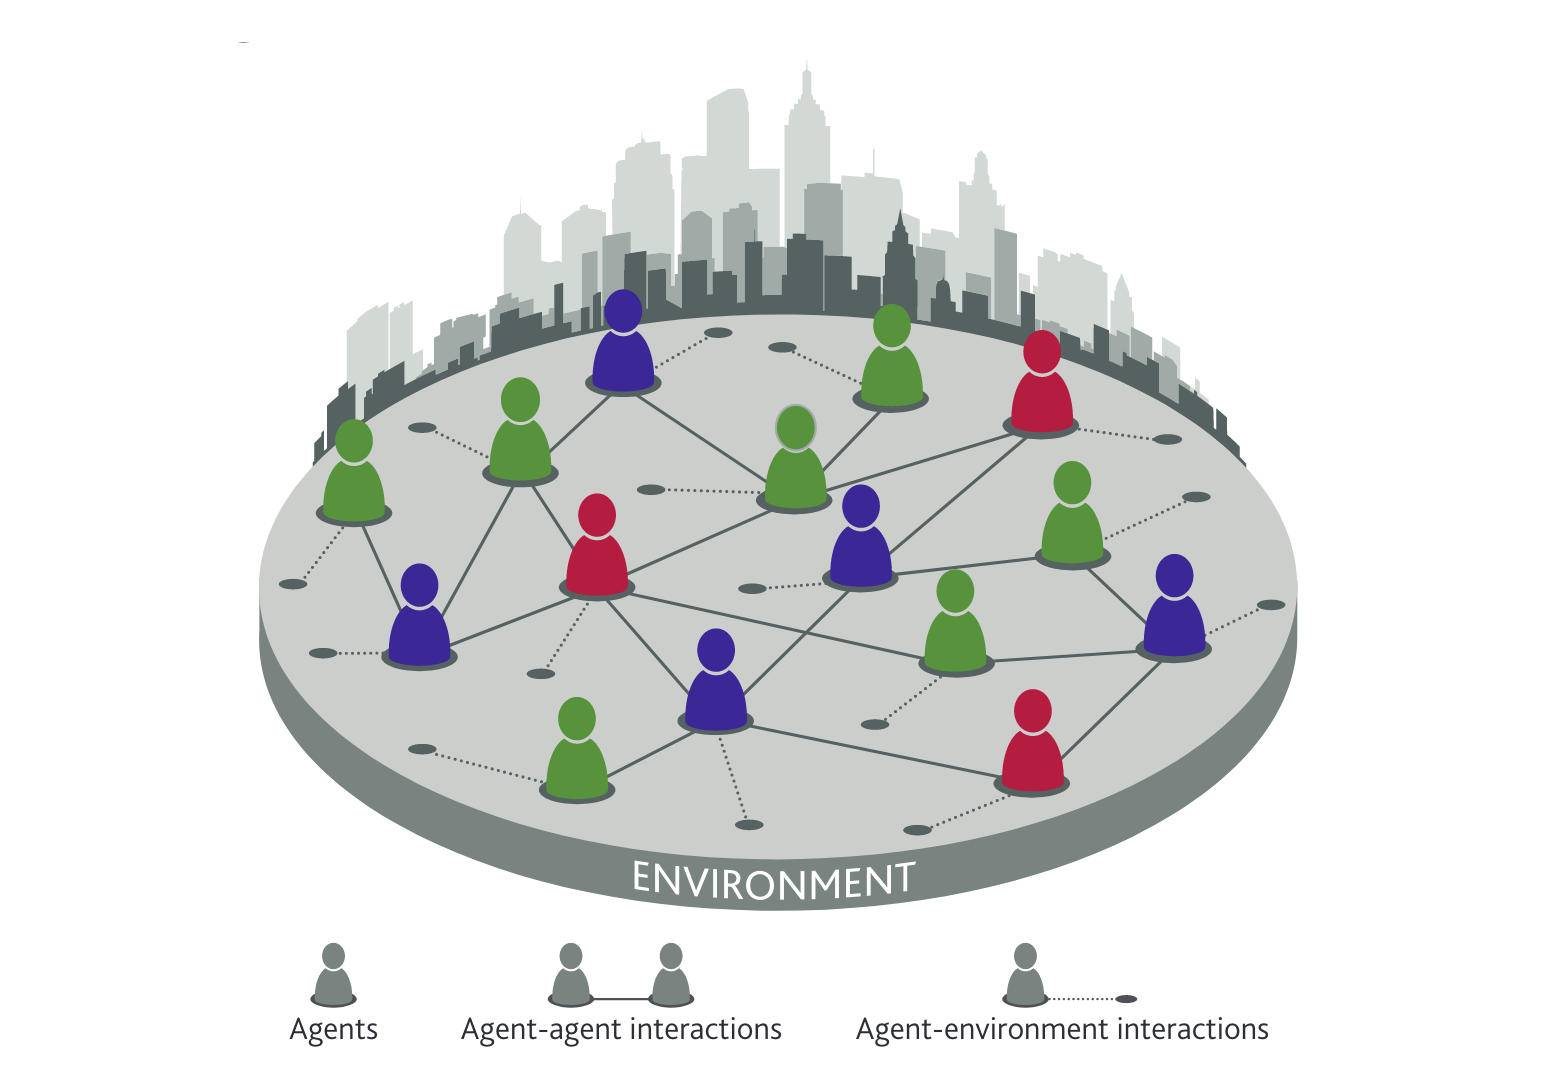
\includegraphics[width=\textwidth]{figs/ABMScheme.png}
        \caption{A schematic of the elements of an agent-based model and their interactions. Source: \cite{haldane_interdisciplinary_2018}.}
    \end{figure}
\end{column}
\end{columns}
\note{\begin{itemize}
        \item Multiple agents with same or different type or behaviour with local information/state. Agents can have very different types such as households, banks or predators/prays.
        \item \textbf{Local} and/or \textbf{global} interaction with other agents or environment. 
        \item Agents make decisions based on their state/information. So even when the behavioural rules are the same of agents, they behave differently depending on their state. Think of these states as information, income, wealth, opinions etc.
        \item Interaction based on \textbf{topology or network}. For instance, an agent can interact with their neighbours or through a network of firms that they know.
        \item Environment in which agents are embedded in. This can be a rectangular grid, a non physical space, or a geographical space where agents can move in.
        \item Global (macro) dynamics are \textbf{emergent} from local (micro) interactions. For instance, GDP growth is caused increase in local sales of items from firms to households.
        \item Expectations are often \textbf{boundedly rational}. Often the economy where the agents live are too complex to even model with rational expectations!
\end{itemize}}
\end{frame}


\begin{frame}{Classic example of agent-based model of \cite{schelling_models_1969}}
\begin{columns}
\begin{column}{0.65\textwidth}
\begin{itemize}
        \item<1-> \textbf{Agent}: Household/consumer/person.
       \item<1-> \textbf{State}: Happiness/utility of the agents.
       \item<2-> \textbf{Action}: If neighbours are not similar enough, the agent moves to an empty spot.
       \item<3-> \textbf{Topology}: Agents interact only with their direct neighbours.
       \item<4-> \textbf{Environment}: The grid where the agents live. In this case, it is rectangular grid.
       \item<5-> Segregation is a \textbf{global phenomenon which emerges from local interactions}.
       \item<6-> Example: \href{https://www.youtube.com/watch?v=dnffIS2EJ30}{Demonstration}
   \end{itemize}
\end{column}
\begin{column}{0.35\textwidth}  
    \begin{figure}
        \centering
        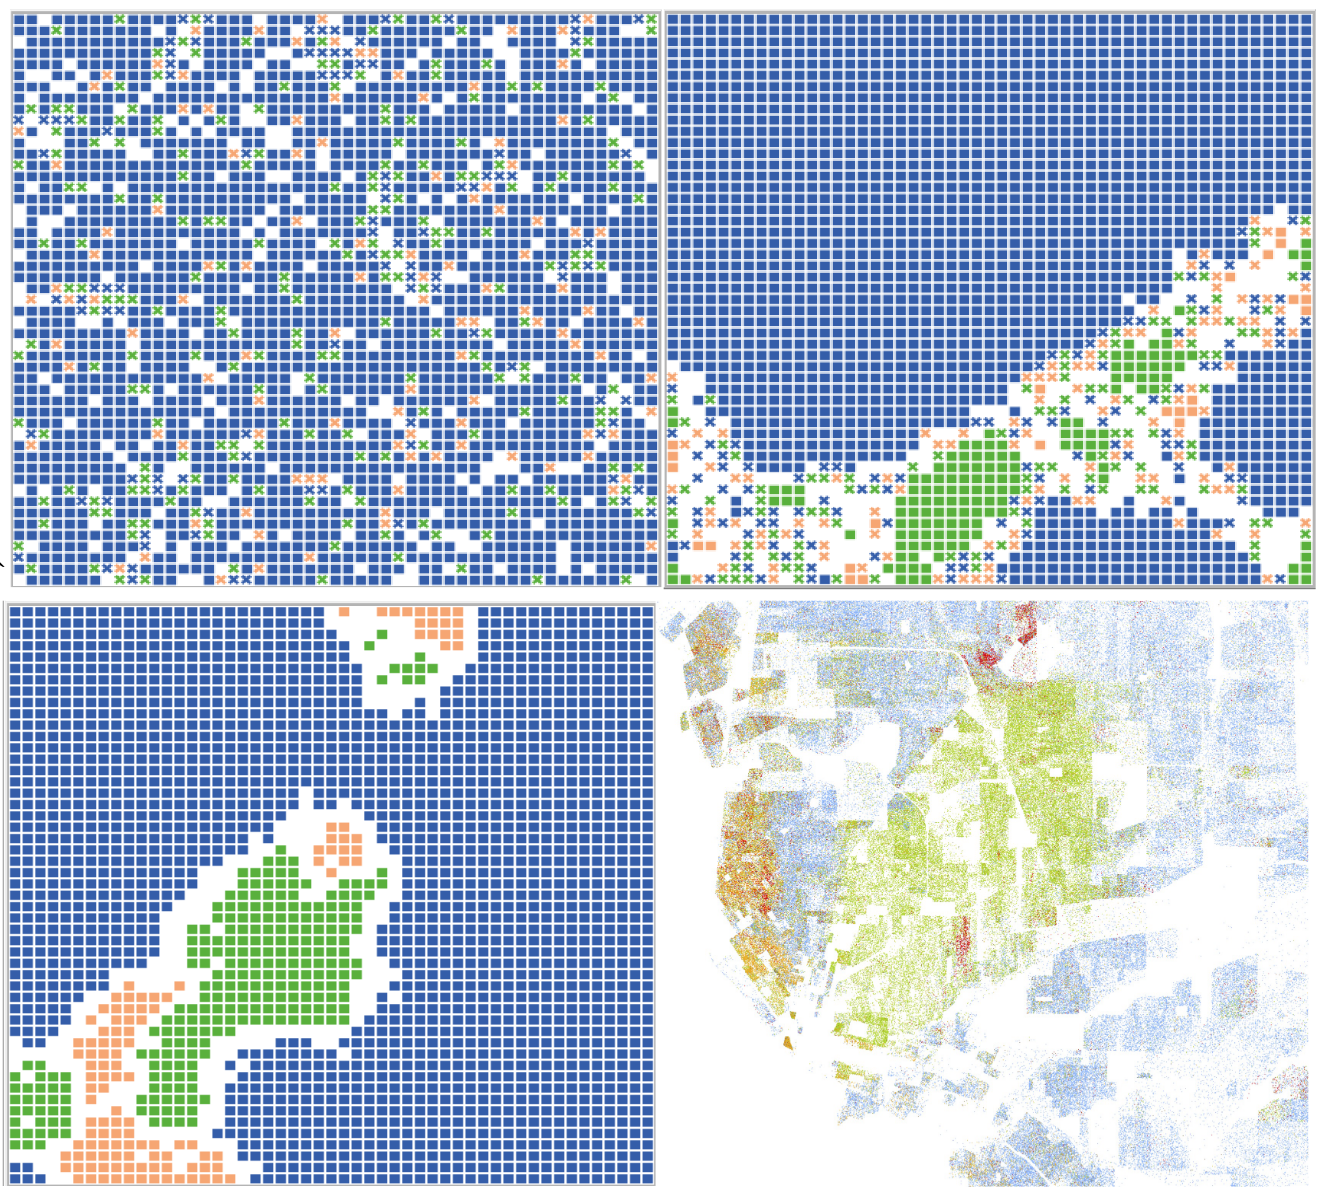
\includegraphics[width =\textwidth]{figs/Schelling.png}
        \caption{One of the first economic agent-based model
       of \cite{schelling_models_1969}. (Source \citep{axtell_agent-based_nodate}}
        \label{fig:schelling}
    \end{figure}
\end{column}
\end{columns}
\note{
\begin{itemize}
       \item \textbf{State}: Happiness/utility of the agents depends on the similarity of neighbours.
       \item \textbf{Action}: If neighbours not similar enough $(\alpha < \underline{\alpha})$, the agents move to an empty spot where at least fraction $\alpha$ of neighbours is similar to me.
       \item \textbf{Topology}: Agents interact only with their direct neighbours.
       \item \textbf{Environment}: The grid where the agents live.
       \item Segregation arises if agents have a slight preference for similarity \citep{schelling_models_1969}. There is a cutoff point of  $\alpha \geq 0.3$ 
       \citep{schelling_models_1969}
       \item Segregation is a \textbf{global phenomenon which emerges from local interactions}.
       \item \href{https://www.youtube.com/watch?v=dnffIS2EJ30}{Demonstration}
   \end{itemize}
}
\end{frame}

\section{ABMs in micro}

\begin{frame}{Simple market in microeconomics}
\begin{columns}
    \begin{column}{0.65\textwidth}  
        \begin{itemize}
            \item<1> There are two parties: Many consumers and suppliers.
            \item<2-> The market clears where the upward-sloping supply curve and downward-sloping demand curve cross.
            \item<3-> It is assumed that some auctioneer has all the information to set a price such that supply equals demand.
            \item<4-> But how does the auctioneer know this?
            \item<5-> In fact, this is extremely difficult! The consumer problem has NP complexity \citep{gilboa_complexity_2021}.
            \item<6-> Where do we see this in real life? 
            \item<7-> Note: Some stylized ABMs like \cite{brock_rational_1997} also assume market equilibrium.
        \end{itemize}
    \end{column}
    \begin{column}{0.4\textwidth}  
        \begin{figure}
            \centering
            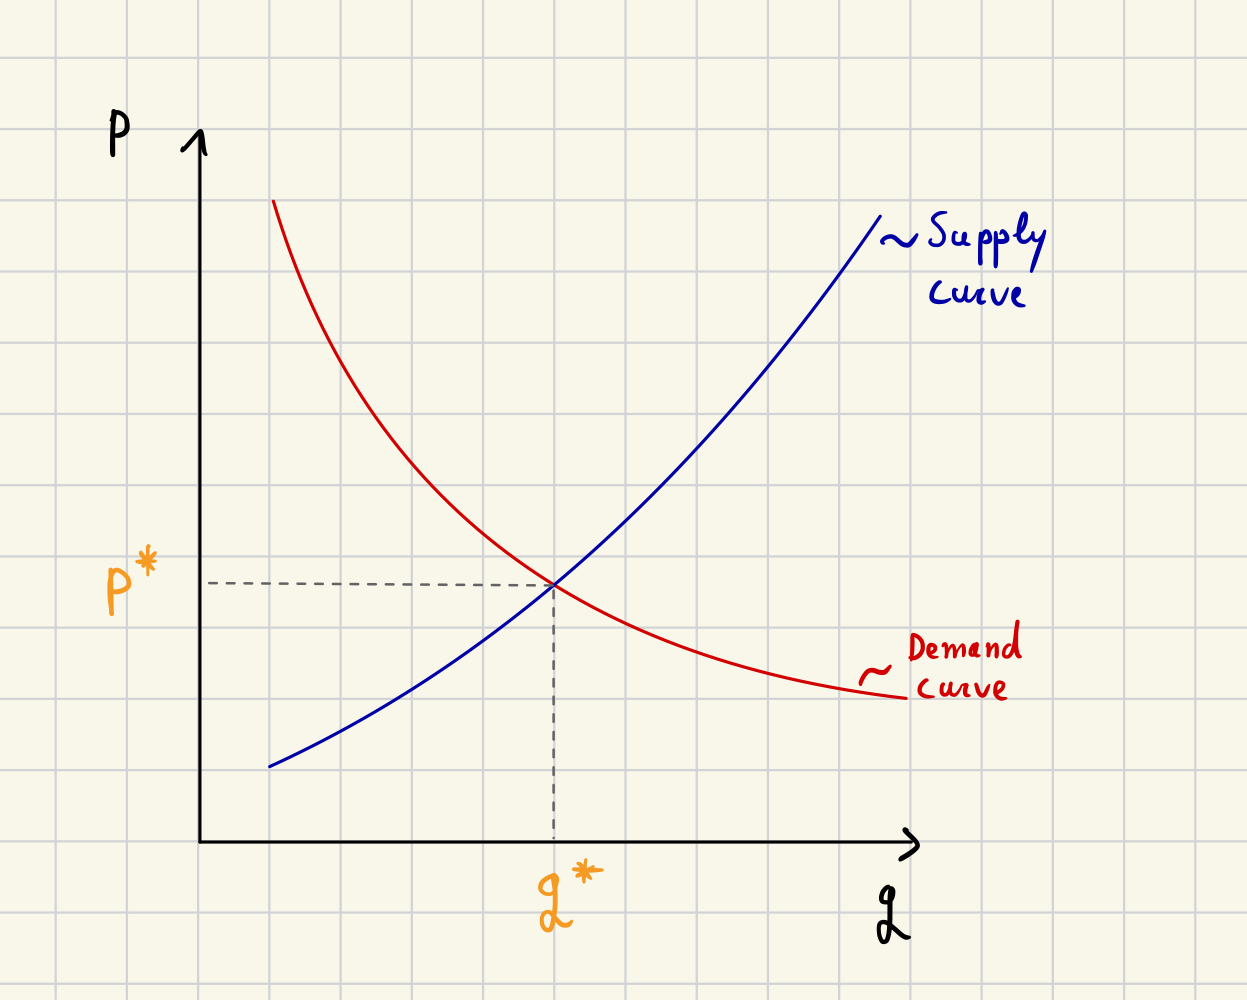
\includegraphics[width=1\textwidth]{figs/micro_equilibrium.jpeg}
            \caption{Microeconomic equilibrium}
            \label{fig:micro_eq}
        \end{figure}
    \end{column}
\end{columns}
\note{\begin{itemize}
            \item Equilibrium occurs where the upward-sloping supply curve and downward-sloping demand curve cross.
            \item It is assumed that some auctioneer has all the information to set a price such that supply equals demand.
            \item But how does the auctioneer know this?
            \item In fact, this is extremely difficult! In fact, the consumer problem has NP complexity \citep{gilboa_complexity_2021}. This means it i
            \item Where do we see this in real life? 
            \item Note: Some stylized ABMs like \cite{brock_rational_1997} also assume market equilibrium.
        \end{itemize}
}
\end{frame}

\begin{frame}{Double Auction Markets}
\begin{columns}
    \begin{column}{0.6\textwidth}
        \begin{itemize}
            \item<1-> Buyers submit bids and sellers submit asks simultaneously based on their valuations.
            \item<2-> A transaction occurs when the bid prices meet or exceed the ask prices.
            \item<3-> No need for an auctioneer.
            \item<5-> Different auction mechanisms also exist, such as:
            \begin{itemize}
                \item<6-> Dutch flower markets 
                \item<7-> English auctions 
                \item<8-> Sealed bid auctions
                \item<9-> Over-the-Counter (OTC) markets
            \end{itemize}
            \item <10-> Simulation example
        \end{itemize}
    \end{column}
    \begin{column}{0.4\textwidth}
        \begin{figure}
            \centering
            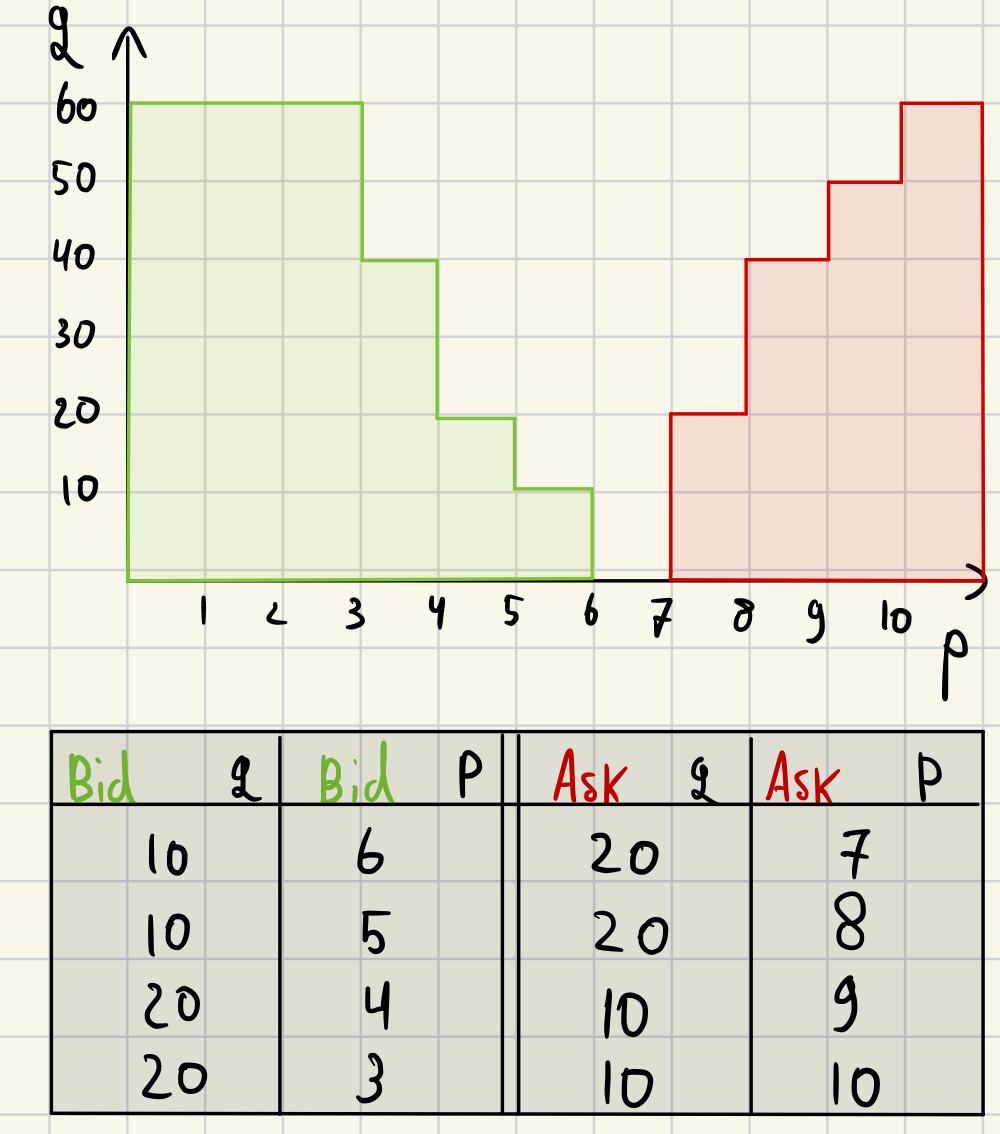
\includegraphics[width=\textwidth]{figs/double_auction.jpeg}
            \caption{Double Auction with bid}
        \end{figure}
    \end{column}
\end{columns}

\note{
    \begin{itemize}
        \item The double auction market is a fundamental mechanism in financial markets and trading platforms.
        \item Buyers and sellers submit their bids and asks simultaneously, making it a decentralized process.
        \item A transaction occurs when a bid meets or exceeds an ask, setting the latest market price.
        \item This process eliminates the need for a central auctioneer but still relies on individual agent interactions.
        \item Variations exist in auction types, such as:
        \begin{itemize}
            \item Dutch auctions, where prices start high and decrease.
            \item English auctions, where prices start low and increase.
            \item Sealed bid auctions, where bids are submitted privately.
            \item OTC markets, which function outside formal exchanges.
        \end{itemize}
        \
    \end{itemize}
}

\end{frame}

\begin{frame}{Decentralized Markets}
\begin{columns}
    \begin{column}{0.7\textwidth}  
        \begin{itemize}
            \item<1-> Markets can be \textbf{decentralized}.
            \item<2-> Buyers or consumers \textbf{search} for firms.
            \item<3-> When a firm is found, whether a sale occurs depends on the price and the availability of the good.
            \item<4-> This is called a \textbf{Search-and-Matching} mechanism.
            \item<4-> This generates a \textbf{bipartite network}
            \item<5-> The seller-buyer network emerges from individual actions.
            \item<6-> Supply does not need to match demand here.
        \end{itemize}
    \end{column}
    \begin{column}{0.4\textwidth}  
        \begin{figure}
            \centering
            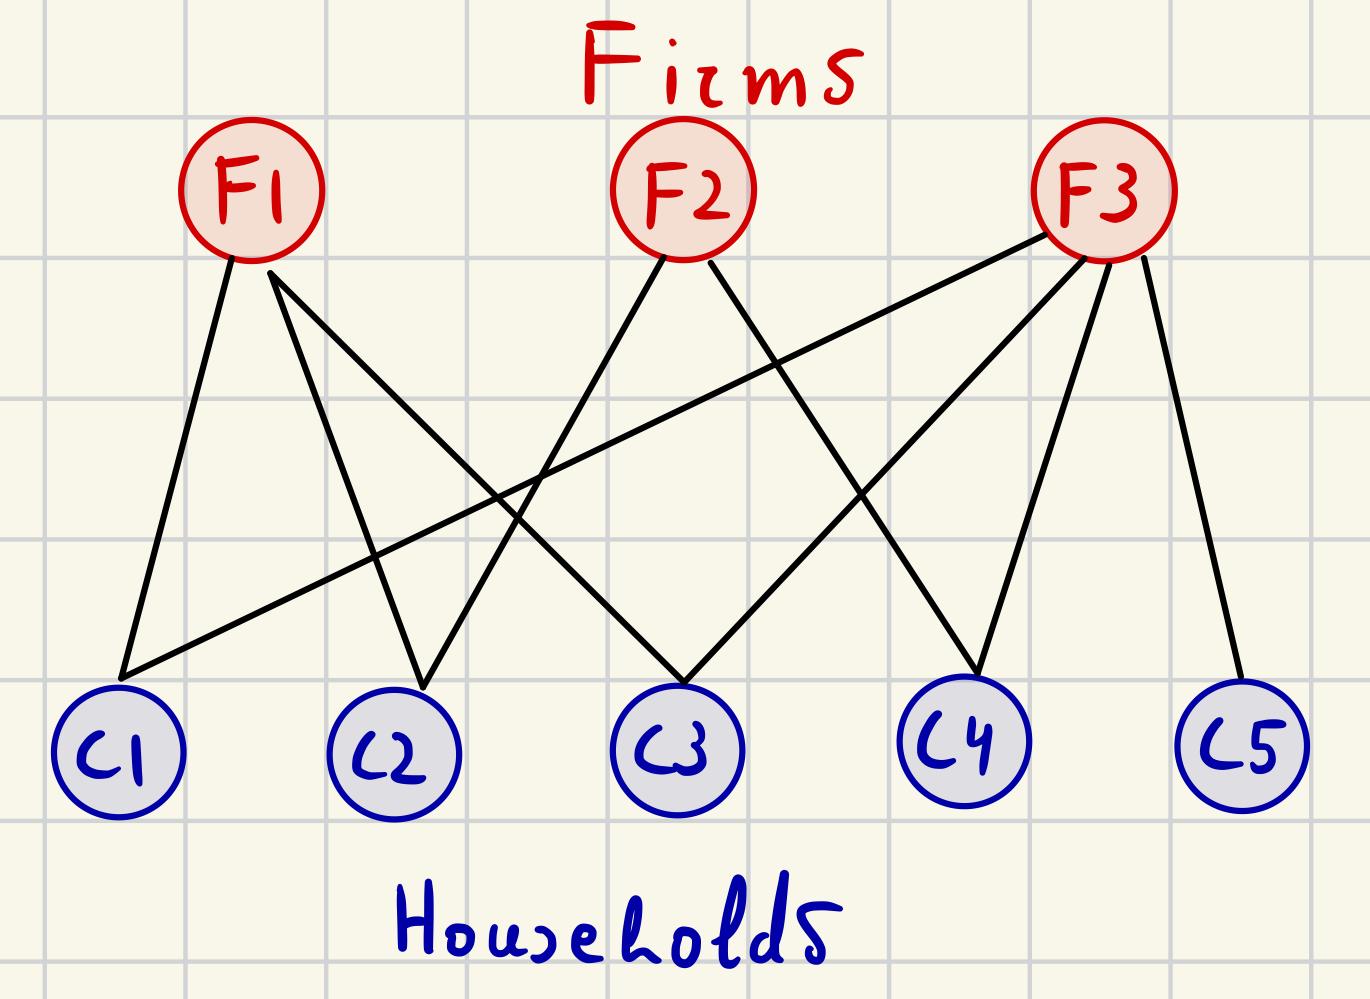
\includegraphics[width=\textwidth]{figs/bipartite_network.jpeg}
            \caption{Decentralized market generated by a search-and-matching mechanism.}
            \label{fig:dec_mar}
        \end{figure}
    \end{column}
\end{columns}

\note{
    \begin{itemize}
        \item Decentralized markets operate without a central auctioneer, meaning that buyers and sellers interact independently.
        \item Buyers must actively search for sellers, which introduces information frictions. They can only check a few firms.
        \item The search process follows specific rules, which can vary based on market structure.
        \item Once a match is found, a transaction may or may not occur, depending on additional market rules.
        \item The seller-buyer network changes dynamically over time based on these interactions.  This can change each period, which can be independent or dependent on the previous network.
        \item Unlike centralized markets, supply and demand do not necessarily have to match at a single price. A distribution of prices of prices can occur.
    \end{itemize}
}

\label{graph_decentralized_markets}
\hyperlink{Market Mechanisms}{\beamerbutton{Go Back}}
\end{frame}

\section{ABMs in Finance}
\begin{frame}{Agent-Based Models (ABMs) in Finance}
    \begin{itemize}
        \item<1-> ABMs can be used to model financial markets and systems.
        \item<2-> We have already seen the double auction market.
        \item<3-> ABMs help explain qualitative financial regularities.
        \item<4-> For example, \cite{brock_rational_1997} developed a stylized agent-based model that:
        \begin{itemize}
            \item<5-> Captured stable asset prices.
            \item<6-> Modeled endogenous bubbles and crashes.
            \item<7-> Explained clustered volatility.
        \end{itemize}
        
    \end{itemize}

\note{
    \begin{itemize}
        \item ABMs provide a flexible way to model financial markets by simulating individual agents with different strategies.
        \item The double auction market example already demonstrated how agent interactions determine price formation.
        \item These models can replicate well-known market features, such as bubbles, crashes, and volatility clustering.
        \item The \cite{brock_rational_1997} model is an early example that paved the way for heterogeneous agent modeling.
        \item The \cite{brock_rational_1997} model initiated a new literature stream on heterogeneous agent models.
        \item These models have been extensively validated empirically \citep{hommes_behavioral_2021}.
    \end{itemize}
}

\end{frame}
\begin{frame}{Banks and Systemic Risk}
    \begin{itemize}
        \item<1-> \cite{eisenberg_systemic_2001} model financial contagion in an interbank network of debt obligations.
        \item<2-> The model represents banks as nodes with obligations to others and operating cash flows.
        \item<3-> It determines a unique "clearing payment vector" that satisfies bankruptcy rules.
        \item<4-> A single bank default can trigger a cascade of defaults through the network.
        \item<5-> The model is static, analyzing a single clearing event rather than an evolving dynamic system.
    \end{itemize}

\note{
    \begin{itemize}
        \item The Eisenberg \& Noe (2001) model is one of the foundational models for studying systemic risk in financial networks.
        
        \item It represents banks as nodes in a network where:
        \begin{itemize}
            \item Each bank has liabilities (debts) to other banks.
            \item Each bank also has operating cash flows to cover these obligations.
        \end{itemize}
        
        \item The model computes a "clearing payment vector", which determines how much each bank pays and whether they meet their obligations. This ensures:
        \begin{itemize}
            \item If a bank has sufficient cash, it repays its obligations fully.
            \item If a bank defaults, repayments are adjusted according to bankruptcy rules.
        \end{itemize}
        
        \item A key insight is that a single default can propagate through the network, triggering a cascade of failures in interconnected banks.
        
        \item The model is static, meaning:
        \begin{itemize}
            \item It focuses on a single moment in time when debts are settled.
            \item It does not capture evolving dynamics like bank reactions, liquidity injections, or policy interventions.
        \end{itemize}
        
        \item This model has been widely applied in:
        \begin{itemize}
            \item Stress-testing financial networks.
            \item Understanding systemic risk in banking crises.
            \item Designing regulatory policies to prevent contagion.
        \end{itemize}
    \end{itemize}
}
\end{frame}
\begin{frame}{Bank balance sheet}
    \begin{columns}
    \begin{column}{0.65\textwidth}  
        \begin{itemize}
            \item<1-> The banks balance sheet consists of the asset side and liability side.
            \item<2-> There are both inside assets and outside asset and inside liabilities and outside liabilities.
            \item<3-> Assets must equal liabilities, hence equity makes up for the difference.
            \item<4-> Can we see how to make a network out of this?
        \end{itemize}
    \end{column}
    \begin{column}{0.35\textwidth}  
        \begin{figure}
            \centering
            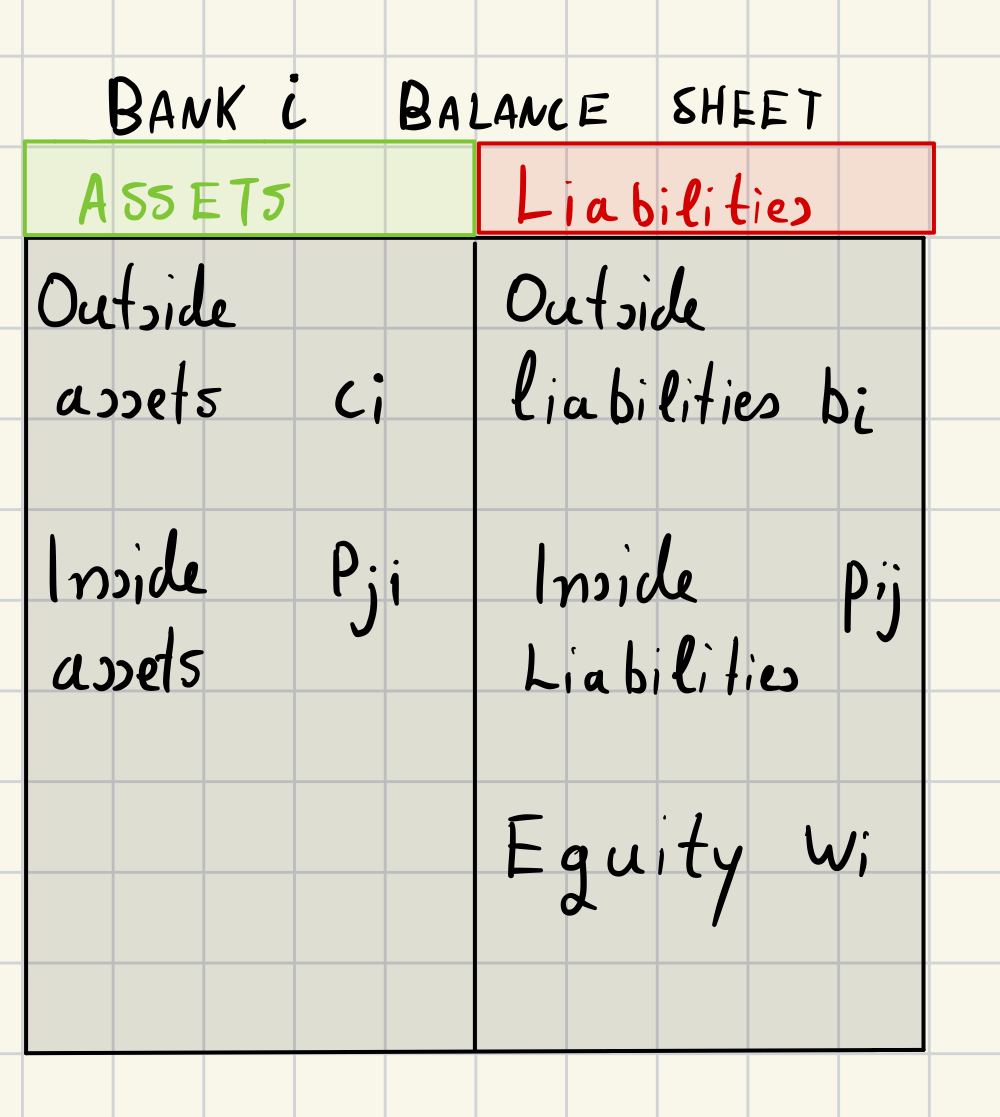
\includegraphics[width=1\linewidth]{figs/Bank_balance_sheet.jpeg}
            \caption{Bank balance sheet for \cite{eisenberg_systemic_2001}}
        \end{figure}
    \end{column}
\end{columns}
\note{\begin{itemize}
    \item Draw a network from bank A, bank B, bank C.
    \item Draw how a 
\end{itemize}}
\end{frame}

\begin{frame}{Systemic Risk and ABMs}
\begin{columns}
    \begin{column}{0.65\textwidth}  
        \begin{itemize}
            \item<1-> \cite{nier_network_2007} extend the Eisenberg and Noe model to study how shocks propagate over multiple rounds.
            \item<2-> The model effectively functions as an agent-based model (ABM) but is not explicitly labeled as one.
            \item<3-> Each bank is represented as a balance sheet that updates based on a clearing rule.
            \item<4-> Monte Carlo simulations explore how changes in structural parameters affect network dynamics.
        \end{itemize}
    \end{column}
    \begin{column}{0.35\textwidth}  
        \begin{figure}
            \centering
            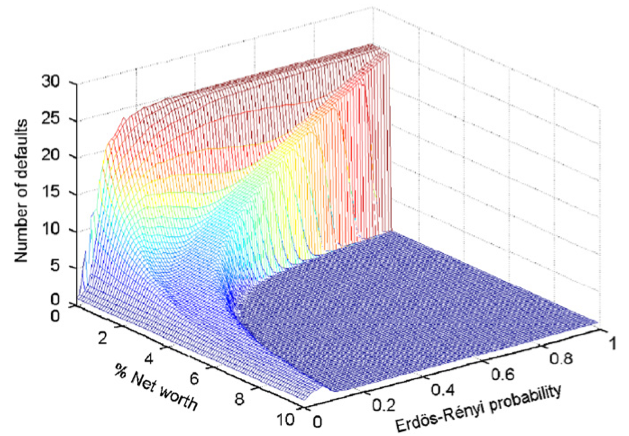
\includegraphics[width=1\linewidth]{figs/defaults.png}
            \caption{Number of defaults as a function of net worth and connectivity probability. Source: \cite{nier_network_2007}}
        \end{figure}
    \end{column}
\end{columns}

\note{
    \begin{itemize}
        \item \cite{nier_network_2007} build upon the Eisenberg \& Noe model but introduce multiple rounds of contagion, making the system dynamic rather than static.
        
        \item Their model behaves like an agent-based model (ABM) because:
        \begin{itemize}
            \item Banks are treated as individual agents with balance sheets that update at each round.
            \item Financial contagion spreads over time rather than in a single clearing event.
        \end{itemize}
        
        \item The model examines:
        \begin{itemize}
            \item How shocks to one or more banks propagate through the network.
            \item How financial network structure affects contagion severity.
        \end{itemize}

        \item A key feature is the use of Monte Carlo simulations, which allow for:
        \begin{itemize}
            \item Testing different network configurations and their resilience to shocks.
            \item Exploring how changes in key parameters (e.g., connectivity, leverage, and liquidity) affect systemic risk.
        \end{itemize}

        \item The results show that:
        \begin{itemize}
            \item Highly interconnected banking systems can spread risk more efficiently but are also more vulnerable to cascades.
            \item Higher capital buffers reduce contagion effects, making the system more stable.
            \item There is a critical threshold where small changes in network structure can lead to significantly higher systemic risk.
        \end{itemize}

        \item This work influenced later agent-based models in systemic risk by demonstrating the importance of dynamic network interactions in financial stability analysis.
    \end{itemize}
}

\end{frame}


\begin{frame}{Going from Qualitative to Quantitative}
    \begin{figure}
        \centering
        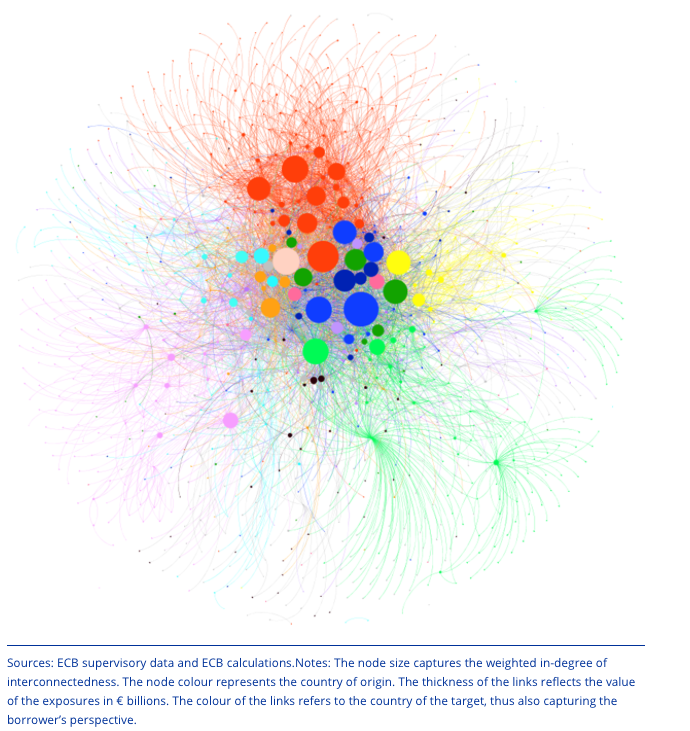
\includegraphics[width=0.55\textwidth]{figs/european_interbank_network.png}
        \caption{Euro area interbank network of large exposures. Source: \cite{covi_economic_2019}}
        \label{European Interbank interbank network of large exposures}
    \end{figure}
\note{\begin{itemize}
    \item Here we can see a visualization of the interbank connectedness of the banks that the ECB visualize.
    \item The model types that I discussed before are now used to analyze how well connected these banks are and how large the systemic risk is.
    \item Stress tests are also done using simulation. For instance, they simulate what happens if suddenly one asset becomes worth less (fire sale) and how this shock propagates through the network.
    \item So these models are now highly relevant for policy analysis!
\end{itemize}}
\end{frame}

\section{ABMs in Macro}


\begin{frame}{Assenza et al. (2015): Model overview}
As a concrete example, consider the model of \cite{assenza_emergent_2015}.
\begin{columns}
\begin{column}{0.5\textwidth}
    \textbf{Agents}
    \begin{itemize}
        \item Households (Worker \& Capitalists)
        \item firms producing consumption goods (C-firms)
        \item firms producing capital goods (K-firms)
        \item banks
    \end{itemize}
    \textbf{Markets}
    \begin{itemize}
        \item Labour (search \& matching)
        \item C goods (search \& matching)
        \item K goods (search \& matching)
        \item Credit (no search \& matching)
        \item Deposits (no search \& matching)
    \end{itemize}
\end{column}
\begin{column}{0.6\textwidth}
        \begin{figure}
        \centering
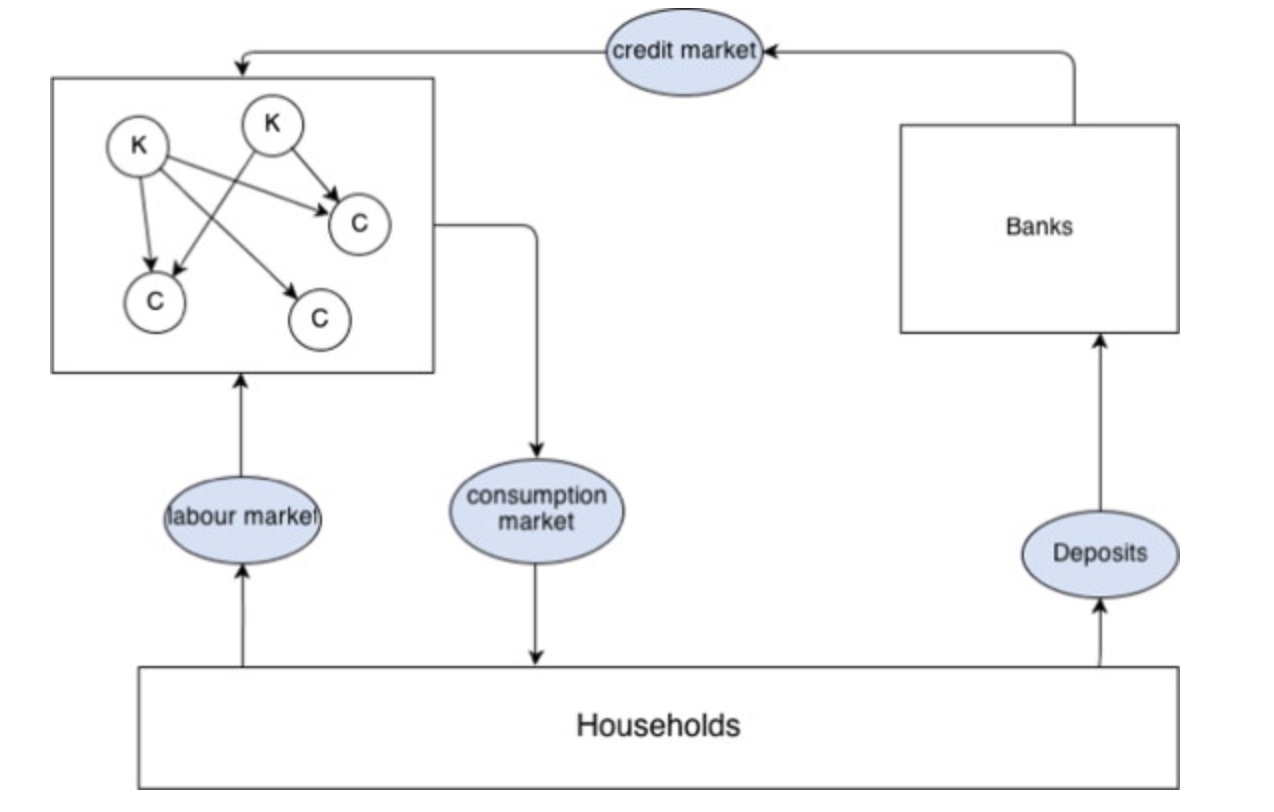
\includegraphics[width=\textwidth]{figs/overview_Assenza_et_al.png}
        \caption{An overview of \cite{assenza_emergent_2015}.}
    \end{figure}
\end{column}
\end{columns}
\end{frame}


\begin{frame}{Households}
\begin{itemize}
  \item \textbf{Labour}: Workers supply one unit of labour inelastically; unemployed workers visit $Z_e$ firms randomly and accept the going wage
  \item \textbf{Income}: Each \textbf{capitalist} owns one firm and receives a share of its profits; workers earn wage $w$
  \item \textbf{Human wealth}: Households form an adaptive estimate of permanent income (exponential moving average of past income)
  \item \textbf{Consumption budget}: Human wealth $+$ a fraction $\chi$ of financial wealth
  \item \textbf{Shopping}: Visit $Z_c$ random C-firms, rank by price, buy from cheapest first
  \item \textbf{Involuntary saving}: If goods are unavailable, unspent budget accumulates as deposits
\end{itemize}
\end{frame}


\begin{frame}{Adaptive Price-Quantity Setting}
Firms do not know their demand curve. They observe two signals, \textbf{inventories} ($\Delta_{i,t}$) and \textbf{relative price} ($P_{i,t}$ vs.\ $\bar{P}_t$), and adjust \emph{either} price \emph{or} quantity:
    \begin{itemize}
            \item Quantity adjustment: $
            Y_{i, t+1}^e= \begin{cases}Y_{i, t}+\rho\left(-\Delta_{i, t}\right) & \text { if } \Delta_{i, t} \leq 0 \text { and } P_{i, t} \geq \bar{P}_t, \\ Y_{i, t}-\rho \Delta_{i, t} & \text { if } \Delta_{i, t}>0 \text { and } P_{i, t}<\bar{P}_t,\end{cases}
            $
            \item Price adjustment: $
            P_{i, t+1}= \begin{cases}P_{i, t}\left(1+\eta_{i, t+1}\right) & \text { if } \Delta_{i, t} \leq 0 \text { and } P_{i, t}<\bar{P}_t, \\ P_{i, t}\left(1-\eta_{i, t+1}\right) & \text { if } \Delta_{i, t}>0 \text { and } P_{i, t} \geq \bar{P}_t,\end{cases}
            $
    \end{itemize}
\vspace{-0.3cm}
\begin{columns}
\begin{column}{0.45\textwidth}
\begin{figure}
    \centering
    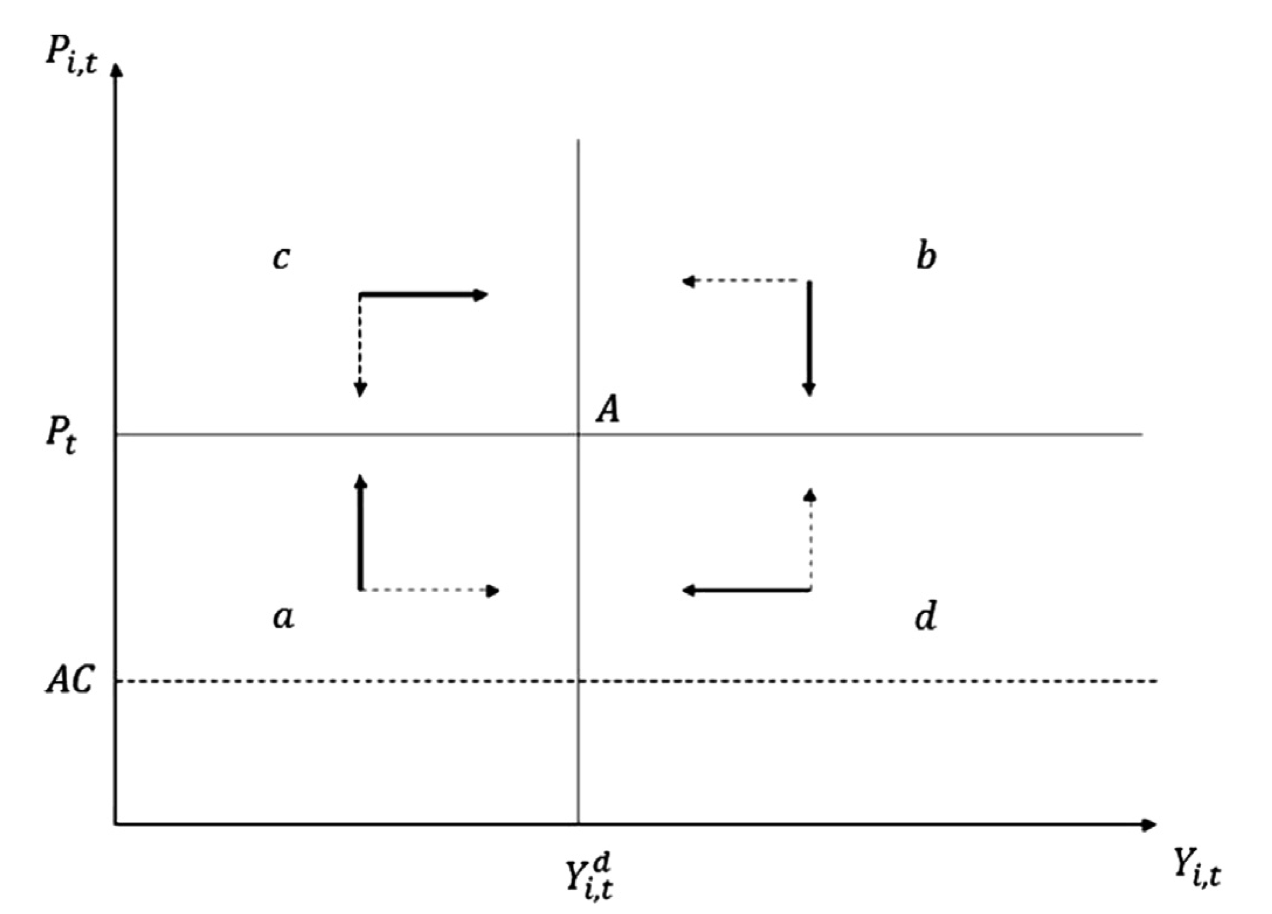
\includegraphics[width=\linewidth]{figs/quantity_price_setting.png}
    \caption{Price-quantity setting. \citep{assenza_emergent_2015}}
\end{figure}
\end{column}
\begin{column}{0.5\textwidth}
\small Both C-firms and K-firms use this mechanism. No firm optimises; each follows a simple heuristic that maps two observable signals to one adjustment.
\end{column}
\end{columns}
\end{frame}

\begin{frame}{Production and Supply Chain}
\begin{columns}[T]
\column{0.48\textwidth}
\textbf{Consumption goods (C-firms)}
\begin{itemize}
  \item Leontief technology:
  $\hat{Y}_{i,t} = \min(\alpha N_{i,t},\; \kappa K_{i,t})$
  \item Uses both \textbf{labour} and \textbf{capital}
  \item Capital depreciates; must be replaced by purchasing from K-firms
  \item If labour or capital unavailable $\Rightarrow$ involuntary underproduction
\end{itemize}

\column{0.48\textwidth}
\textbf{Capital goods (K-firms)}
\begin{itemize}
  \item Linear technology: $Y_{j,t} = \alpha N_{j,t}$ (labour only)
  \item Upstream supplier: output is a durable, storable input for C-firms
  \item Same adaptive price-quantity mechanism
\end{itemize}

\vspace{0.3cm}
\textbf{Key point}
\begin{itemize}
  \item Two-sector supply chain creates \textbf{interdependence}: C-firms depend on K-firms for capital; K-firms depend on C-firm investment demand
\end{itemize}
\end{columns}
\end{frame}


\begin{frame}{Credit and Financial Accelerator}
\begin{itemize}
  \item Firms borrow to cover the \textbf{financing gap}: production costs that exceed internal funds
  \item The bank sets interest rates based on \textbf{leverage} $\lambda = \text{debt}/\text{equity}$
  \item The bank \textbf{rations credit} when expected losses exceed its risk tolerance
\end{itemize}

\vspace{0.15cm}
\begin{columns}[T]
\begin{column}{0.48\textwidth}
\centering
\textbf{\small Financial Accelerator}\\[0.15cm]
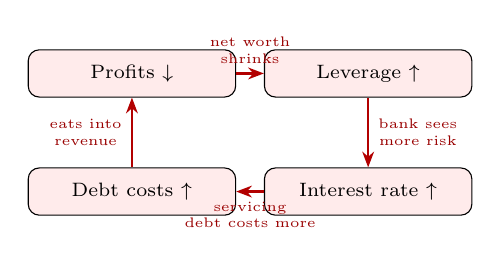
\begin{tikzpicture}[
  box/.style={rectangle, draw, rounded corners, fill=red!8, text width=2.4cm, align=center, font=\scriptsize, minimum height=0.6cm},
  arr/.style={-{Stealth[length=2mm]}, thick, red!70!black},
  lbl/.style={font=\tiny, text=red!60!black, align=center}]
\node[box] (prof) at (0, 0) {Profits $\downarrow$};
\node[box] (lev) at (3, 0) {Leverage $\uparrow$};
\node[box] (rate) at (3, -1.5) {Interest rate $\uparrow$};
\node[box] (cost) at (0, -1.5) {Debt costs $\uparrow$};
\draw[arr] (prof) -- node[lbl, above] {net worth\\shrinks} (lev);
\draw[arr] (lev) -- node[lbl, right] {bank sees\\more risk} (rate);
\draw[arr] (rate) -- node[lbl, below] {servicing\\debt costs more} (cost);
\draw[arr] (cost) -- node[lbl, left] {eats into\\revenue} (prof);
\end{tikzpicture}
\end{column}
\begin{column}{0.48\textwidth}
\centering
\textbf{\small Bank Capital Channel}\\[0.15cm]
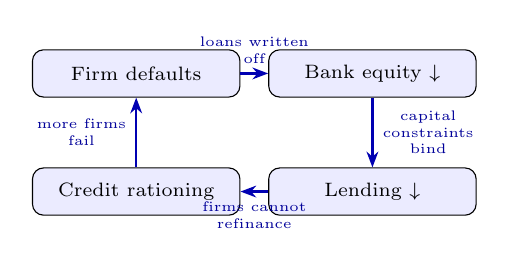
\begin{tikzpicture}[
  box/.style={rectangle, draw, rounded corners, fill=blue!8, text width=2.4cm, align=center, font=\scriptsize, minimum height=0.6cm},
  arr/.style={-{Stealth[length=2mm]}, thick, blue!70!black},
  lbl/.style={font=\tiny, text=blue!60!black, align=center}]
\node[box] (def) at (0, 0) {Firm defaults};
\node[box] (eq) at (3, 0) {Bank equity $\downarrow$};
\node[box] (lend) at (3, -1.5) {Lending $\downarrow$};
\node[box] (ration) at (0, -1.5) {Credit rationing};
\draw[arr] (def) -- node[lbl, above] {loans written\\off} (eq);
\draw[arr] (eq) -- node[lbl, right] {capital\\constraints\\bind} (lend);
\draw[arr] (lend) -- node[lbl, below] {firms cannot\\refinance} (ration);
\draw[arr] (ration) -- node[lbl, left] {more firms\\fail} (def);
\end{tikzpicture}
\end{column}
\end{columns}

\vspace{0.15cm}
\centering
\small These loops amplify small shocks into large swings and generate instability \textbf{endogenously}.
\end{frame}

\begin{frame}{Emergent Crises}
How does the model generate crises \textbf{without exogenous shocks}?

\vspace{0.1cm}
\centering
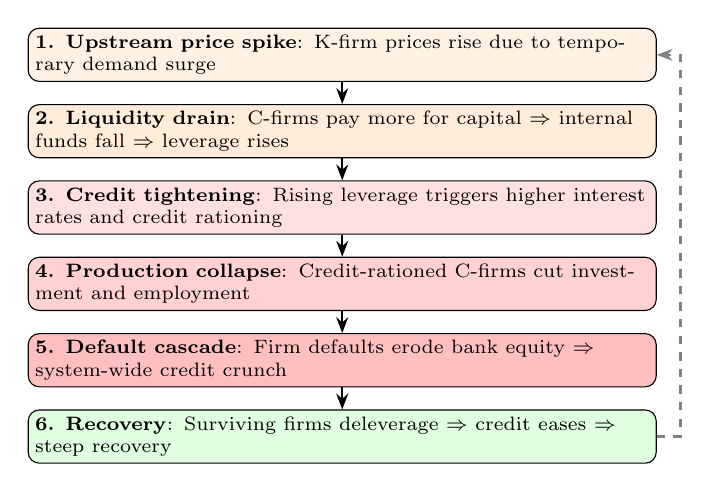
\begin{tikzpicture}[
  box/.style={rectangle, draw, rounded corners, text width=7.8cm, align=left, font=\scriptsize, minimum height=0.4cm, inner sep=2.5pt},
  arr/.style={-{Stealth[length=2mm]}, thick},
  node distance=0.28cm]
\node[box, fill=orange!10] (s1) {\textbf{1. Upstream price spike}: K-firm prices rise due to temporary demand surge};
\node[box, fill=orange!15, below=of s1] (s2) {\textbf{2. Liquidity drain}: C-firms pay more for capital $\Rightarrow$ internal funds fall $\Rightarrow$ leverage rises};
\node[box, fill=red!12, below=of s2] (s3) {\textbf{3. Credit tightening}: Rising leverage triggers higher interest rates and credit rationing};
\node[box, fill=red!18, below=of s3] (s4) {\textbf{4. Production collapse}: Credit-rationed C-firms cut investment and employment};
\node[box, fill=red!25, below=of s4] (s5) {\textbf{5. Default cascade}: Firm defaults erode bank equity $\Rightarrow$ system-wide credit crunch};
\node[box, fill=green!12, below=of s5] (s6) {\textbf{6. Recovery}: Surviving firms deleverage $\Rightarrow$ credit eases $\Rightarrow$ steep recovery};

\draw[arr] (s1) -- (s2);
\draw[arr] (s2) -- (s3);
\draw[arr] (s3) -- (s4);
\draw[arr] (s4) -- (s5);
\draw[arr] (s5) -- (s6);
\draw[arr, dashed, gray] (s6.east) -- ++(0.3, 0) |- (s1.east);
\end{tikzpicture}

\vspace{0.1cm}
\small\textbf{Key insight}: No exogenous shock is needed; the supply chain and credit feedback loops are sufficient.
\end{frame}

\begin{frame}{Simulation Results}
\begin{figure}
    \centering
    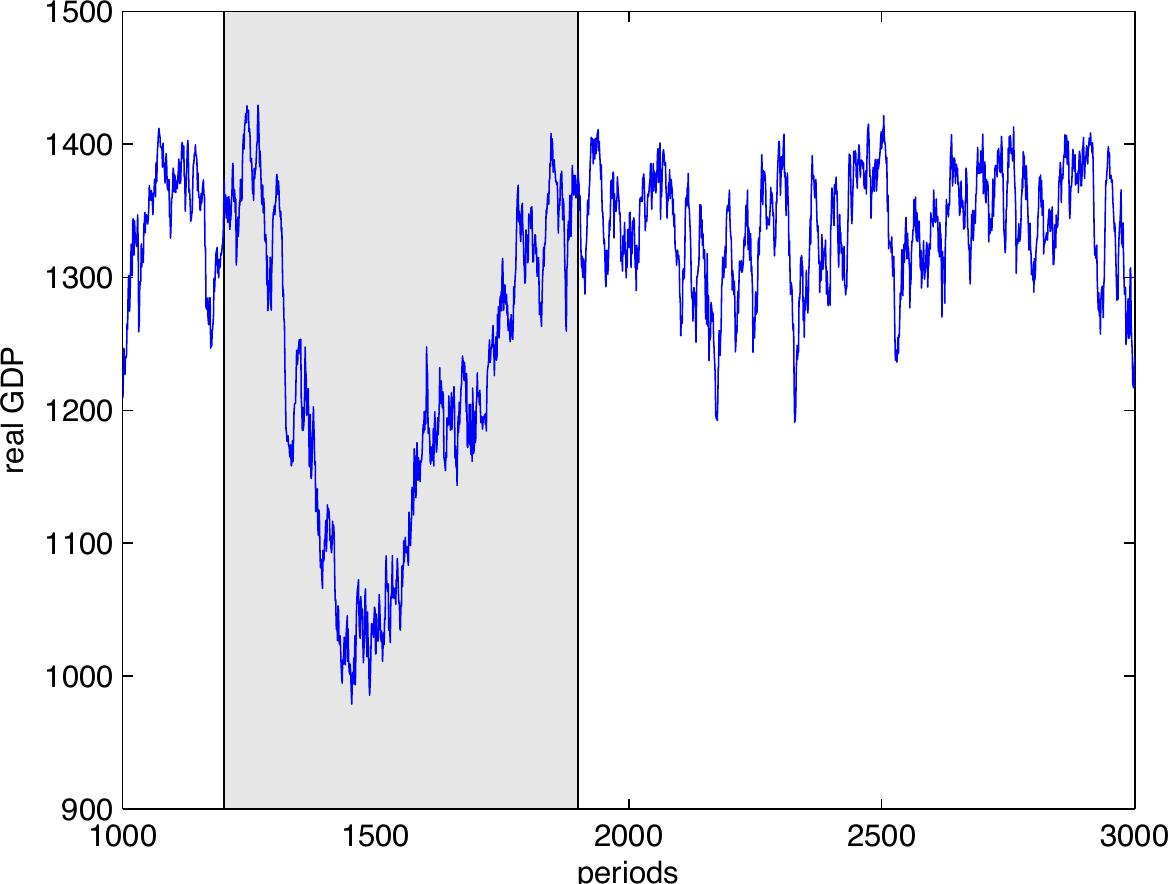
\includegraphics[width=0.85\linewidth]{figs/simulation_results_assenza.png}
    \caption{Simulated output of \cite{assenza_emergent_2015}. Deep recessions emerge endogenously from the interaction of the supply chain and credit feedback.}
\end{figure}
\end{frame}

\begin{frame}{Validation}
\begin{columns}
\begin{column}{0.5\textwidth}
    \begin{figure}
        \centering
        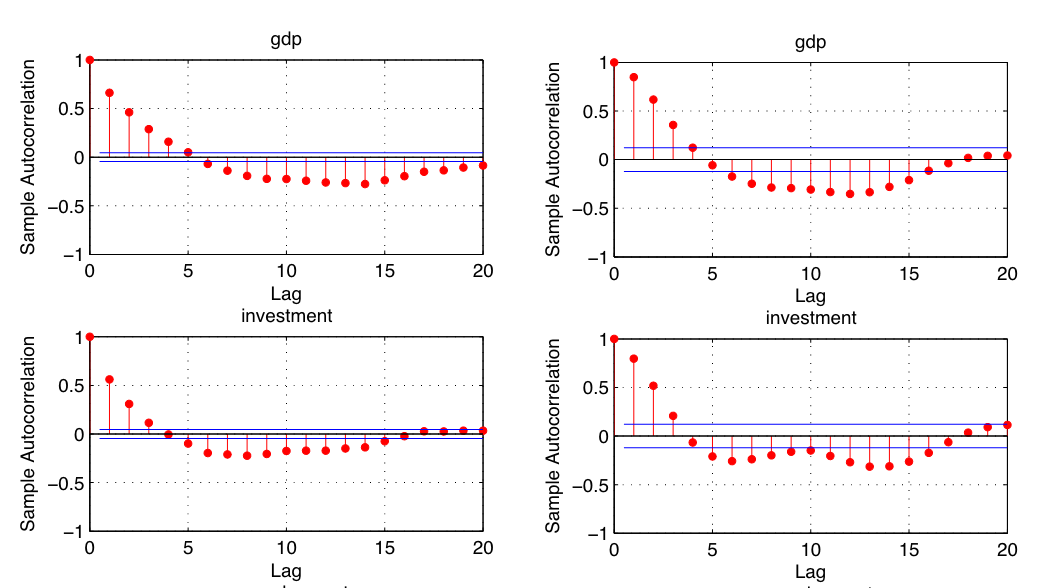
\includegraphics[width=\linewidth]{figs/Autocorrelations1.png}
        \caption{Autocorrelations: model (left) vs.\ data (right). \citep{assenza_emergent_2015}}
    \end{figure}
\end{column}
\begin{column}{0.5\textwidth}
    \begin{figure}
        \centering
        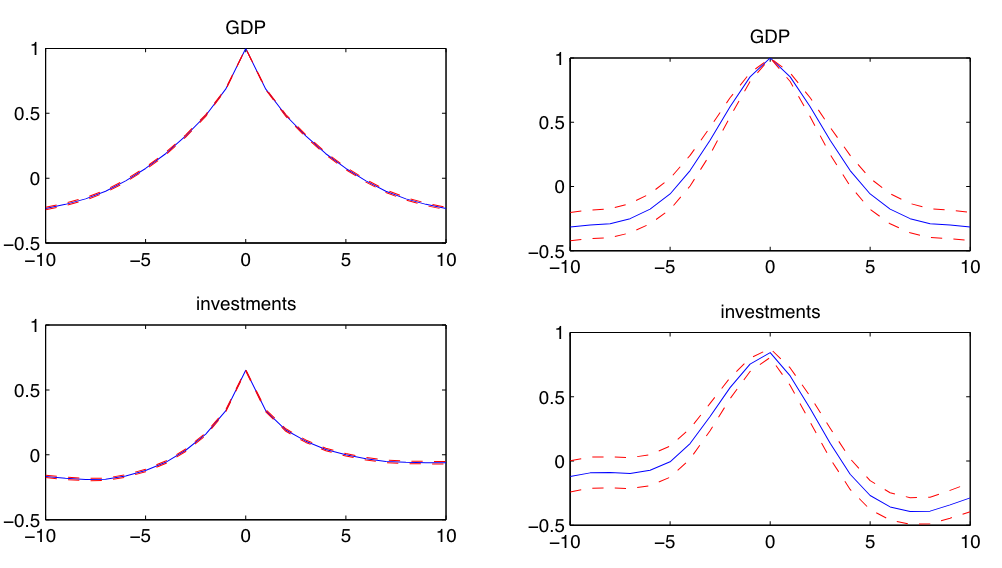
\includegraphics[width=\linewidth]{figs/correlations1.png}
        \caption{Correlations: model (left) vs.\ data (right). \citep{assenza_emergent_2015}}
    \end{figure}
\end{column}
\end{columns}
\vspace{0.2cm}
The model reproduces key empirical regularities, persistence (high autocorrelation) and co-movement patterns, without relying on exogenous shocks.
\end{frame}

\begin{frame}{\cite{assenza_emergent_2015} summary}
\begin{columns}[T]
\begin{column}{0.48\textwidth}
\textbf{Model Structure:}
\begin{itemize}
\item Two-sector economy:
  \begin{itemize}
  \item Upstream: Capital goods producers
  \item Downstream: Consumption goods firms
  \end{itemize}
\item Adaptive behavior for price/quantity decisions
\item Banking sector with credit constraints
\end{itemize}

\textbf{Key Findings:}
\begin{itemize}
\item Business cycles emerge without external shocks
\item Reproduces empirical time series properties
\item Crises occur from sectoral interactions
\end{itemize}
\end{column}

\begin{column}{0.48\textwidth}
\textbf{Crisis Mechanism:}
\begin{itemize}
\item Spike in capital goods prices
\item Consumption firms increase borrowing
\item Credit rationing emerges when debt is high
\item Production contracts, causing recession
\item Recovery follows deleveraging
\end{itemize}

\textbf{Implications:}
\begin{itemize}
\item Upstream-downstream dynamics matter
\item Debt cycles drive business cycles
\item Adaptive behavior creates persistence
\end{itemize}
\end{column}
\end{columns}
\end{frame}


\begin{frame}{Overview}
    \begin{itemize}
        \item<1-> Agent based models (ABMs) are simulation-based modelling approach where agents interact.
        \item<2-> We covered some of the general properties that ABMs have.
        \item<3-> We looked at examples of ABMs in microeconomics, finance, and macroeconomics.
        \item<4-> We walked through the \cite{assenza_emergent_2015} model as a concrete macro ABM example.
        \item<5-> Next time: quantitative ABMs calibrated to real data, and calibration techniques.
        \item<6-> For now a little demonstration with \textit{BeforeIT}.jl and \textit{ABCcredit}.jl packages which are really well developed Julia packages to get you working with qualitative and quantitative ABMs.
    \end{itemize}
\end{frame}
\begin{frame}
    \Huge \centering \textbf{Questions?}
\end{frame}
\begin{frame}[allowframebreaks]{Bibliography}
    \bibliography{example}
\end{frame}

\end{document}
